%
\documentclass[11pt, oneside]{article}      % use 'amsart' instead of 'article' for AMSLaTeX format
\usepackage{geometry}                       % See geometry.pdf to learn the layout options. There are lots.
\geometry{letterpaper}                      % ... or a4paper or a5paper or ...
%\geometry{landscape}                       % Activate for for rotated page geometry
\usepackage[parfill]{parskip}               % Activate to begin paragraphs with an empty line rather than an indent
\usepackage{graphicx}                       % Use pdf, png, jpg, or eps with pdflatex; use eps in DVI mode
                                            % TeX will automatically convert eps --> pdf in pdflatex
\usepackage{amssymb}
%\date{\today}                              % Activate to display a given date or no date
\title{Structure of pHs \texttt{BJTAMP}}
%
\usepackage{authblk}
\usepackage{hyperref}
%\renewcommand\Authands{ and }
%
%
\author[1]{Antoine Falaize}
%
\author[2]{John Doe}
%
\affil[1]{Project-team S3\footnote{\url{http://s3.ircam.fr}}, \\STMS, IRCAM-CNRS-UPMC (UMR 9912), \\1 Place Igor-Stravinsky, 75004 Paris, France}
%
\affil[2]{Project-team S3\footnote{\url{http://s3.ircam.fr}}, \\STMS, IRCAM-CNRS-UPMC (UMR 9912), \\1 Place Igor-Stravinsky, 75004 Paris, France}
%
\begin{document}
%
\maketitle
%
%
\section{System netlist}
%
%
\begin{center}
%
\texttt{
\begin{tabular}{llllll}
\hline
line & label & dictionary.component & nodes &     parameters \\ \hline
%
$\ell_1$ & IN & electronics.source & ('IN', 'ref') & $\left\{ 
%
\begin{tabular}{ll}
%
type & voltage
\\
\end{tabular}\right.$
 \\
$\ell_2$ & Cin & electronics.capacitor & ('IN', '5') & $\left\{ 
%
\begin{tabular}{ll}
%
C & ('Cin', 1e-05)
\\
\end{tabular}\right.$
 \\
$\ell_3$ & Rbc & electronics.resistor & ('5', '6') & $\left\{ 
%
\begin{tabular}{ll}
%
R & ('Rbc', 270000.0)
\\
\end{tabular}\right.$
 \\
$\ell_4$ & BJT & electronics.bjt & ('5', '6', 'ref') & $\left\{ 
%
\begin{tabular}{ll}
%
mu & ('mu', 1.006)
\\
betaF & ('betaF', 294.3)
\\
Vt & ('Vt', 0.026)
\\
betaR & ('betaR', 7.946)
\\
Rb & ('Rb', 1)
\\
Rc & ('Rc', 0.85)
\\
Is & ('Is', 2.39e-14)
\\
Re & ('Re', 0.4683)
\\
\end{tabular}\right.$
 \\
$\ell_5$ & Rcd & electronics.resistor & ('vcc', '6') & $\left\{ 
%
\begin{tabular}{ll}
%
R & ('Rcd', 1000.0)
\\
\end{tabular}\right.$
 \\
$\ell_6$ & VCC & electronics.source & ('vcc', 'ref') & $\left\{ 
%
\begin{tabular}{ll}
%
type & voltage
\\
\end{tabular}\right.$
 \\
$\ell_7$ & Cout & electronics.capacitor & ('OUT', '6') & $\left\{ 
%
\begin{tabular}{ll}
%
C & ('Cout', 1e-05)
\\
\end{tabular}\right.$
 \\
$\ell_8$ & OUT & electronics.source & ('OUT', 'ref') & $\left\{ 
%
\begin{tabular}{ll}
%
type & current
\\
\end{tabular}\right.$
 \\
\hline
\end{tabular}
%
}
%
\end{center}
%
    %
    \begin{figure}[!h]
    \begin{center}
    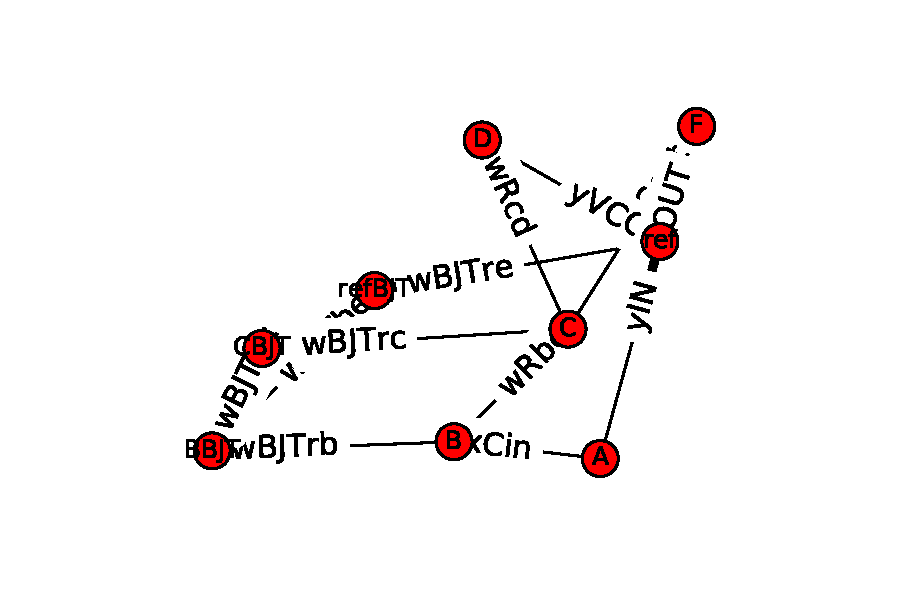
\includegraphics[width=\linewidth]{/Users/Falaize/Documents/DEV/python/pyphs/tests/BJTAMP/figures/BJTAMP_graph.pdf}
    %
    \caption{\label{fig:graph_BJTAMP} Graph of system \texttt{BJTAMP}. }
    \end{center}
    \end{figure}
    %\section{System dimensions}
%
$\dim(\mathbf{x})=$ $ n_\mathbf{x} = 2 ; $ 
%
\\
%
$\dim(\mathbf{w})=$ $ n_\mathbf{w} = 7 ; $ 
%
\\
%
$\dim(\mathbf{y})=$ $ n_\mathbf{y} = 3 ; $ 
%
\\
%
$\dim(\mathbf{p})=$ $ n_\mathbf{p} = 0 ; $ 
%
\\
%
%
\section{System variables}
%
State variable $ \mathbf{x} = \left(\begin{array}{c}x_{\mathrm{Cin}}\\x_{\mathrm{Cout}}\end{array}\right) ; $ 
%
\\
%
Dissipation variable $ \mathbf{w} = \left(\begin{array}{c}w_{\mathrm{Rcd}}\\w_{\mathrm{BJTbe}}\\w_{\mathrm{BJTbc}}\\w_{\mathrm{BJTre}}\\w_{\mathrm{BJTrc}}\\w_{\mathrm{BJTrb}}\\w_{\mathrm{Rbc}}\end{array}\right) ; $ 
%
\\
%
Input $ \mathbf{u} = \left(\begin{array}{c}u_{\mathrm{IN}}\\u_{\mathrm{VCC}}\\u_{\mathrm{OUT}}\end{array}\right) ; $ 
%
\\
%
Output $ \mathbf{y} = \left(\begin{array}{c}y_{\mathrm{IN}}\\y_{\mathrm{VCC}}\\y_{\mathrm{OUT}}\end{array}\right) ; $ 
%
\\
%
%
\section{Constitutive relations}
%
Hamiltonian $ \mathtt{H}(\mathbf{x}) = \frac{0.5}{\mathrm{Cout}} \cdot x_{\mathrm{Cout}}^{2} + \frac{0.5}{\mathrm{Cin}} \cdot x_{\mathrm{Cin}}^{2} ; $ 
%
\\
%
Hamiltonian gradient $ \nabla \mathtt{H}(\mathbf{x}) = \left(\begin{array}{c}\frac{1.0}{\mathrm{Cin}} \cdot x_{\mathrm{Cin}}\\\frac{1.0}{\mathrm{Cout}} \cdot x_{\mathrm{Cout}}\end{array}\right) ; $ 
%
\\
%
Dissipation function $ \mathbf{z}(\mathbf{w}) = \left(\begin{array}{c}\frac{w_{\mathrm{Rcd}}}{\mathrm{Rcd}}\\- \mathrm{Is} \cdot \left(e^{\frac{w_{\mathrm{BJTbc}}}{\mathrm{Vt} \cdot \mathrm{mu}}} - 1\right) - 1.0 \cdot 10^{-9} \cdot w_{\mathrm{BJTbc}} + \frac{1}{\mathrm{betaF}} \cdot \left(\mathrm{betaF} + 1\right) \cdot \left(\mathrm{Is} \cdot \left(e^{\frac{w_{\mathrm{BJTbe}}}{\mathrm{Vt} \cdot \mathrm{mu}}} - 1\right) + 1.0 \cdot 10^{-9} \cdot w_{\mathrm{BJTbe}}\right)\\- \mathrm{Is} \cdot \left(e^{\frac{w_{\mathrm{BJTbe}}}{\mathrm{Vt} \cdot \mathrm{mu}}} - 1\right) - 1.0 \cdot 10^{-9} \cdot w_{\mathrm{BJTbe}} + \frac{1}{\mathrm{betaR}} \cdot \left(\mathrm{betaR} + 1\right) \cdot \left(\mathrm{Is} \cdot \left(e^{\frac{w_{\mathrm{BJTbc}}}{\mathrm{Vt} \cdot \mathrm{mu}}} - 1\right) + 1.0 \cdot 10^{-9} \cdot w_{\mathrm{BJTbc}}\right)\\\mathrm{Re} \cdot w_{\mathrm{BJTre}}\\\mathrm{Rc} \cdot w_{\mathrm{BJTrc}}\\\mathrm{Rb} \cdot w_{\mathrm{BJTrb}}\\\mathrm{Rbc} \cdot w_{\mathrm{Rbc}}\end{array}\right) ; $ 
%
\\
%
Jacobian of dissipation function $ \mathcal{J}_{\mathbf{z}}(\mathbf{w}) = \left(\begin{array}{ccccccc}\frac{1}{\mathrm{Rcd}} & 0 & 0 & 0 & 0 & 0 & 0\\0 & \frac{1}{\mathrm{betaF}} \cdot \left(\mathrm{betaF} + 1\right) \cdot \left(\frac{\mathrm{Is} \cdot e^{\frac{w_{\mathrm{BJTbe}}}{\mathrm{Vt} \cdot \mathrm{mu}}}}{\mathrm{Vt} \cdot \mathrm{mu}} + 1.0 \cdot 10^{-9}\right) & - \frac{\mathrm{Is} \cdot e^{\frac{w_{\mathrm{BJTbc}}}{\mathrm{Vt} \cdot \mathrm{mu}}}}{\mathrm{Vt} \cdot \mathrm{mu}} - 1.0 \cdot 10^{-9} & 0 & 0 & 0 & 0\\0 & - \frac{\mathrm{Is} \cdot e^{\frac{w_{\mathrm{BJTbe}}}{\mathrm{Vt} \cdot \mathrm{mu}}}}{\mathrm{Vt} \cdot \mathrm{mu}} - 1.0 \cdot 10^{-9} & \frac{1}{\mathrm{betaR}} \cdot \left(\mathrm{betaR} + 1\right) \cdot \left(\frac{\mathrm{Is} \cdot e^{\frac{w_{\mathrm{BJTbc}}}{\mathrm{Vt} \cdot \mathrm{mu}}}}{\mathrm{Vt} \cdot \mathrm{mu}} + 1.0 \cdot 10^{-9}\right) & 0 & 0 & 0 & 0\\0 & 0 & 0 & \mathrm{Re} & 0 & 0 & 0\\0 & 0 & 0 & 0 & \mathrm{Rc} & 0 & 0\\0 & 0 & 0 & 0 & 0 & \mathrm{Rb} & 0\\0 & 0 & 0 & 0 & 0 & 0 & \mathrm{Rbc}\end{array}\right) ; $ 
%
\\
%
%
\section{System parameters}
%
%
\subsection{Constant}
%
\begin{center}
%
\begin{tabular}{ll}
%
\hline
parameter & value (SI)
\\ \hline
betaF :& 294.3
\\
Rbc :& 270000.0
\\
betaR :& 7.946
\\
Rb :& 1
\\
Rcd :& 1000.0
\\
Re :& 0.4683
\\
Vt :& 0.026
\\
Cin :& 1e-05
\\
mu :& 1.006
\\
Is :& 2.39e-14
\\
Cout :& 1e-05
\\
Rc :& 0.85
\\
\hline
\end{tabular}
%
\end{center}
%
$ \mathbf{J} = \left(\begin{array}{cccccccccccc}0 & 0 & -1.0 & 1.0 & 0 & 0 & 0 & 0 & 0 & 0 & 0 & 1.0\\0 & 0 & 0 & 0 & 0 & 0 & 0 & 0 & 0 & 0 & 0 & -1.0\\1.0 & 0 & 0 & 0 & 0 & 0 & 0 & 0 & 1.0 & -1.0 & 1.0 & 0\\-1.0 & 0 & 0 & 0 & 0 & 1.0 & 0 & -1.0 & 0 & 1.0 & 0 & 0\\0 & 0 & 0 & 0 & 0 & 0 & 1.0 & -1.0 & 1.0 & 0 & 0 & 0\\0 & 0 & 0 & -1.0 & 0 & 0 & 0 & 0 & 0 & 0 & 0 & 0\\0 & 0 & 0 & 0 & -1.0 & 0 & 0 & 0 & 0 & 0 & 0 & 0\\0 & 0 & 0 & 1.0 & 1.0 & 0 & 0 & 0 & 0 & 0 & 0 & 0\\0 & 0 & -1.0 & 0 & -1.0 & 0 & 0 & 0 & 0 & 0 & 0 & 1.0\\0 & 0 & 1.0 & -1.0 & 0 & 0 & 0 & 0 & 0 & 0 & 0 & -1.0\\0 & 0 & -1.0 & 0 & 0 & 0 & 0 & 0 & 0 & 0 & 0 & 0\\-1.0 & 1.0 & 0 & 0 & 0 & 0 & 0 & 0 & -1.0 & 1.0 & 0 & 0\end{array}\right) ; $ 
%
\\
%
\end{document}